\scanpage{33}
donc $c_{\ell,i+j}$ et $c_{\ell+j,i}\not\equiv0\ (p)$. C'est le contenu du

\uline{Lemme 2} Soient $i,j\geq0$. Alors il existe $\ell\geq0$ tel que $\deleted{\unsure{c_{ij\ell}}}c_{i+j,\ell}$ et $c_{i,j+\ell}$ soient $\not\equiv0\ (p)$.
\figure{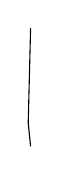
\begin{tikzpicture}\draw (0,0)--(-.03,-1.2)--(0,-1.5);\end{tikzpicture}}

\deleted{\uline{Dém} Considérons les développements $p$-adiques de $i$ et $j$
\[
i=i_0+i_1p+\cdots+i_rp^r
\]
\[
j=j_0+j_1p+\cdots+j_rp^r
\]
alors le développement $p$-adique de $\inserted{\sigma=}i+j$ est
\inserted{$\deleted{\unsure{i+}}j=\sigma=\sigma_0+\sigma_1p+\cdots+\sigma_{r+1}p^{r+1}$}
donné par le procédé \unsure{vraiment|couramment} bien connu, où on détermine par récurrence les couples d'entiers $\sigma_\alpha,\deleted{\unsure{\rho_\alpha}}$ $(0\leq\alpha\leq r+1)$ \inserted{et $\rho_\alpha$ $(-1\leq\alpha\leq r)$} --- les $\rho_\alpha$ sont les ``retenues'', égales à $0$ ou $1$ --- en posant \deleted{$\unsure{\rho_0=0}$}
\[
\textcircled{a}\quad\rho_{-1}=0,
\]
puis par récurrence par
\inserted{$0\leq\alpha\leq r$}
\[
\textcircled{b}\quad i_\alpha+j_\alpha+\rho_{\alpha-1}=\sigma_\alpha+p\rho_\alpha\qquad0\leq\sigma_\alpha,\rho_\alpha\leq p-1
\]
\margin{celà détermine $\sigma_\alpha$ et $\rho_\alpha$}
enfin
\[
\textcircled{c}\quad\sigma_{\unsure{\alpha|r}+1}=\rho_{\unsure{r}}
\]
Posons
\[
\ell_\alpha=(p-1)-\sigma_\alpha\qquad0\leq\alpha\leq r+1
\]
\[
\ell=\sum_0^{r+1}\ell_\alpha p^\alpha
\]
d'où $\sigma+\ell=\sum_0^{r+1}(p-1)p^\alpha=p^{r+2}-1$ i.e. $\ell=p^{r+2}-1-\sigma$.
On a alors, grâce à (b)
\[
\textcircled{a'}\quad\rho_{-1}=0
\]
\[
\textcircled{b'}\quad\text{Si }0\leq\alpha\leq r,\qquad(i_\alpha+j_\alpha+\ell_\alpha)+\rho_{\alpha-1}=(p-1)+p\rho_\alpha
\]
\margin{(où $\rho_{\alpha-1}$ et $\rho_\alpha$ sont $0\leq\ \leq p-1$)}
\[
\textcircled{b'}\mathrm{bis}\quad\deleted{\unsure{\alpha}}\underset{\substack{\text{''}\\0}}{i_{r+1}}+\underset{\substack{\text{''}\\0}}{j_{r+1}}+\ell_{r+1}+\rho_r=(p-1)+p.0
\]
\deleted{$\textcircled{c'}\quad\unsure{i_{r+1}+j_{r+1}}$}
Ce qui montre que \deleted{\unsure{inject.}} l'addition de}
\mspage{32}
